%% =====================================================================
%%  The Constraint Layer
%%  Autonomous agents, deterministic ledgers, and the missing
%%  substrate of machine consequence
%%
%%  Build:  pdflatex main.tex  (run twice)   |  arXiv-ready, TeX Live
%% =====================================================================
\pdfoutput=1
\documentclass[11pt]{article}

\usepackage[margin=1in]{geometry}
\usepackage[T1]{fontenc}
\usepackage[utf8]{inputenc}
\usepackage{lmodern}
\usepackage{microtype}
\usepackage{amsmath,amssymb}
\usepackage{booktabs}
\usepackage{graphicx}
\usepackage{caption}
\usepackage{enumitem}
\usepackage{xcolor}
\usepackage[numbers,sort&compress]{natbib}
\usepackage[colorlinks=true,linkcolor=black,citecolor=black,
            urlcolor={blue!35!black}]{hyperref}
\usepackage{xurl}

\captionsetup{font=small,labelfont=bf,width=0.94\textwidth}
\setlist{itemsep=2pt,topsep=4pt}
\emergencystretch=1.5em

\hypersetup{
  pdftitle={The Constraint Layer: Autonomous Agents, Deterministic
            Ledgers, and the Missing Substrate of Machine Consequence},
  pdfauthor={Xinhao Zheng},
  pdfsubject={autonomous agents; verifiable computation; deterministic
              settlement; zero-knowledge; blockchain; delegation},
}

\newcommand{\R}[1]{R#1}

\title{\textbf{The Constraint Layer:\\[3pt]
  Autonomous Agents, Deterministic Ledgers, and the\\
  Missing Substrate of Machine Consequence}}
\author{%
  Xinhao Zheng\thanks{Correspondence: \texttt{xinhaozheng.vx@outlook.com}.
    Code and data:
    \url{https://github.com/xinhao-zheng/constraint-layer}.}\\[2pt]
  \small Independent Researcher}
\date{12 June 2026}

\begin{document}
\maketitle

\begin{abstract}
\noindent
An autonomous software agent can now decide, but it cannot bind. A
current model will plan a transaction, draft a contract, or instruct a
payment, yet nothing it emits is by itself accountable: its behaviour is
non-deterministic, it holds no stake, it cannot prove that it stayed
within the authority it was given, and it cannot make any outcome
irreversible. The deficit is structural rather than a matter of scale---
more capable models decide better; they do not thereby become bindable.
We argue that the missing faculty---rule-bound, provable, settleable
consequence---is precisely what a particular kind of public ledger
supplies, and that the two are complements rather than competitors:
generative systems are open-ended and unconstrained exactly where
ledgers are rigid and rule-governed, and each is of little use to
consequential autonomy without the other. We give the anatomy of the
gap; state the five properties a ledger must hold to act as a
\emph{constraint layer} for agents---provably secure consensus;
deterministic settlement under which a locally checked action equals the
globally settled one; proofs expressive enough to carry private
compliance predicates; an economy that funds neutrality without an
owner; and rules that can amend themselves---and show why the dominant
ledger designs satisfy at most some of them. We then read one deployed
architecture against the five as a case study, in design terms rather
than market terms, and describe the form agent commerce takes once
authority is compiled into a checkable policy and settlement doubles as
audit. Two technologies usually filed together as a fad are in fact the
two halves of one missing primitive: machines that decide, and a
substrate on which their decisions can carry consequence. The decision
is becoming abundant; the consequence is not; and building the second is
the harder, and the more neglected, half.
\end{abstract}

\paragraph*{Keywords.} autonomous agents; verifiable computation;
deterministic settlement; zero-knowledge proofs; smart contracts;
delegation; AI safety.

\section{Introduction}
\label{sec:intro}

The hard problem of an autonomous agent is not that it might think
poorly. It is that it can act without being bound. A language model wired
to tools will read a market, choose a counterparty, size a position, and
issue the instruction to move funds---and at no point in that sequence is
there anything that holds it to what it was permitted to do, records what
it actually did in a form a stranger can check, or makes the result
final. Capability research is pouring effort into the first half of
autonomy, the deciding. The second half, the part that lets a decision
\emph{count}, has no comparable program, because it was never a property
of the model in the first place.

That second half has a name in economics it predates: the machinery by
which parties who do not trust each other can nonetheless transact.
Institutions exist to lower the cost of doing so
\citep{north1990institutions}, and trust is the lubricant that lets the
whole system move \citep{arrow1974limits}. For human actors the machinery
is ambient---contracts, registries, courts, reputations, the threat of
consequence---and an autonomous agent inherits none of it. It has no
reputation that a bad act would damage, no assets a court could reach, no
identity that persists with liability across runs. The literature on
agentic systems has catalogued the resulting hazards
\citep{park2023generative,chan2023harms}; we read them as symptoms of a
single absence. An agent is a faculty of decision without a faculty of
consequence.

This article makes three moves. First (\S\ref{sec:gap}), it gives the
anatomy of that absence: the specific, structural things an agent lacks
the moment its decisions are supposed to bind other parties---and argues
that none of them is closed by making the model larger. Second
(\S\ref{sec:complement}--\S\ref{sec:requirements}), it identifies the
complement. A public ledger of the right kind is not another decider
competing with the model; it is a substrate of consequence---
deterministic where the agent is non-deterministic, rule-governed where
the agent is open-ended, able to make an outcome provable and final where
the agent can only assert. The fit is close enough to look designed: the
agent supplies what the ledger cannot (open-ended decision), the ledger
supplies what the agent cannot (bound, provable, settled consequence).
But ``a ledger'' is not enough; only a ledger with five specific
properties can hold an agent without reintroducing the trusted third
party it was meant to remove, and the best-known designs hold at most
some of the five. Third (\S\ref{sec:case}--\S\ref{sec:commerce}), it
reads one deployed architecture against those five requirements as a
worked case---on documented design, not market performance---and
describes the shape commerce takes when an agent's authority is compiled
into a predicate its counterparties can check and settlement is itself
the audit trail.

The claim is deliberately narrow and falsifiable in form. It is not that
blockchains are good, or that any token will appreciate; the case study
(\S\ref{sec:case}) is explicit that architecture is not adoption, and
\S\ref{sec:open} states what would refute the thesis. The claim is that
the pairing of generative decision with verifiable, deterministic
consequence is a genuine technical direction rather than a slogan, that
it is forced by the way autonomy is arriving, and that most of the
engineering difficulty lives on the consequence side, which the present
enthusiasm for ever-larger deciders is not addressing.

\section{The Unbound Agent}
\label{sec:gap}

What, precisely, does an autonomous agent lack the instant its outputs
are meant to move money, bind a counterparty, or carry legal weight?
Six things, none of them an intelligence deficit.

\paragraph{Non-determinism.}
A model's output is a sample, not a function. Re-run it and the answer
can change; the same is not acceptable of a payment or a contract
execution, where the property required is that the operation mean exactly
one thing and that any observer recompute it identically. Determinism is
not a quality a more capable sampler converges to; it is a different
regime, and consequential action lives only inside it.

\paragraph{No rule-binding by construction.}
An agent can be \emph{told} a rule---a spending limit, an allowed
counterparty set, a jurisdictional constraint---and may, probabilistically,
respect it. There is no level on which the rule is binding rather than
advisory. Guardrails written in the same medium as the behaviour they
constrain are suggestions; what consequential delegation needs is a rule
the agent \emph{cannot} violate because the violation is rejected
elsewhere, not merely discouraged within the model.

\paragraph{No proof of its own conduct.}
After the fact, an agent cannot demonstrate that it acted within its
mandate; it can only assert it, and its assertion is exactly the kind of
fluent, unfalsifiable artifact that machine generation now produces
without cost. Detecting misconduct after the fact by inspecting outputs
is, in the limit, unreliable: classifier-based detection of generated
content decays toward chance as models improve
\citep{sadasivan2023detection}, and strong watermarking admits generic
removal under plausible assumptions \citep{zhang2023watermarks}. Trust
that must be reconstructed from the agent's own testimony is no trust at
all.

\paragraph{No bounded, delegable authority.}
To hand an agent authority today is to hand it a credential---an API key,
a wallet seed---that is effectively unbounded: whoever holds it can do
whatever the underlying account can do. There is no native way to grant
\emph{this much and no more} such that the bound is enforced by the
counterparty rather than hoped for by the principal. Delegation without
an enforceable boundary is not delegation; it is abdication.

\paragraph{No settlement.}
An agent can compute that a transfer should happen; it cannot make it
\emph{have happened}. Finality---the point past which an action cannot be
silently undone or reordered---is a property of a settlement system, not
of a reasoner. Without it, every downstream party must price the risk
that what the agent ``did'' will be revised, and that risk is a tax on
every interaction.

\paragraph{No accountable identity.}
Asked ``what is this, and who stands behind it?'' an agent has no
structural answer. It is not a person, holds nothing at risk, and its
relationship to whatever principal deployed it is, to a counterparty,
unverifiable. The oldest informal verification---ask, and watch the
answers cohere---now selects for better generators, not honest actors.

These are not failures of cognition, and they do not shrink as cognition
grows; a model twice as capable decides better and is no more bindable.
They are failures of \emph{consequence}: of the agent's inability to make
its decisions rule-bound, provable, final, and attributable. Each is the
mirror image of a property that one specific class of system has been
engineering for a decade and a half.
\section{The Deterministic Complement}
\label{sec:complement}

The properties an agent lacks are the defining properties of a public
ledger. This is not a coincidence to be admired but a complementarity to
be used: the two systems are strong in exactly disjoint places.
Generative models are open-ended, creative, and unconstrained, and they
have no rules until someone supplies them; ledgers are rigid,
rule-governed, and deterministic, and everything they do is about proof
and provability. Neither is sufficient for autonomy that carries
consequence. A ledger decides nothing---it is inert without an actor to
propose actions. An agent settles nothing---it is unaccountable without a
substrate to make actions bind. Put the generativity on one side and the
bindability on the other (Figure~\ref{fig:complement}a) and the design
target is the upper-right region neither occupies alone: an agent that
proposes, on a substrate that binds.

\begin{figure}[t]
  \centering
  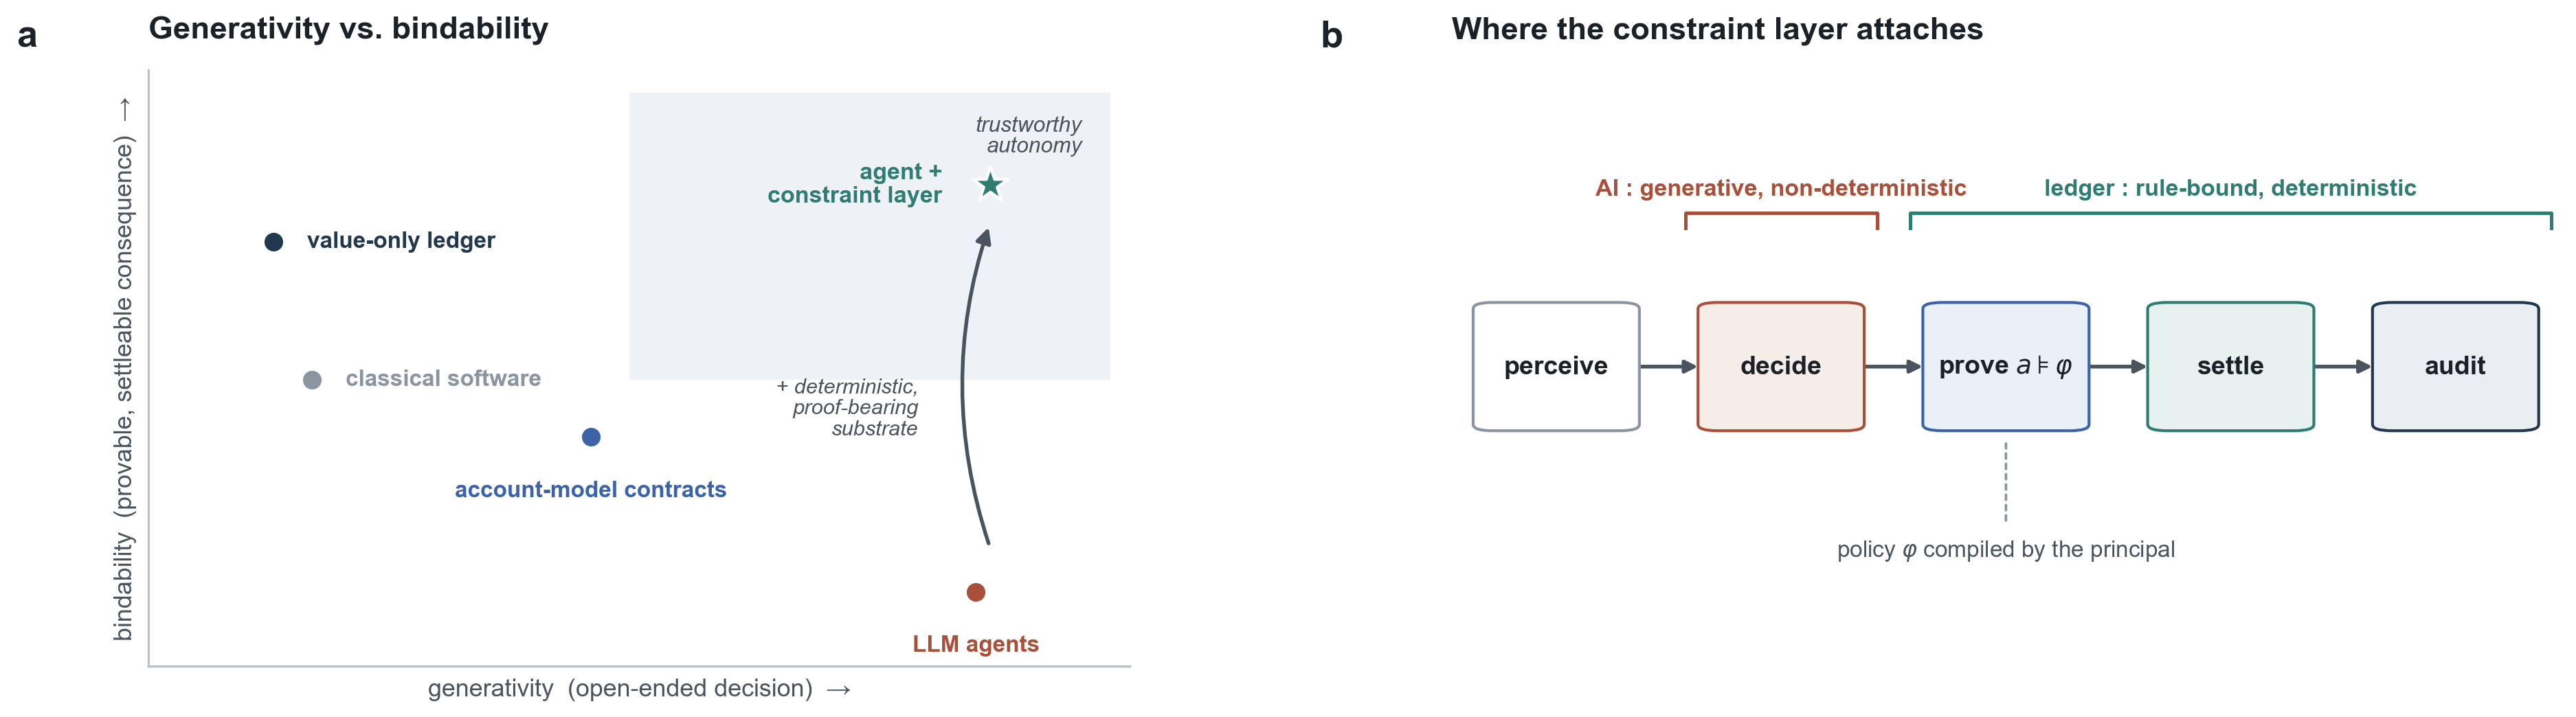
\includegraphics[width=\textwidth]{fig1_complementarity.png}
  \caption{The complementarity. \textbf{(a)}~Systems placed by
    \emph{generativity} (capacity for open-ended decision) against
    \emph{bindability} (capacity to make a decision provable, settleable,
    and final). Generative agents sit at high generativity and near-zero
    bindability; value-only and account-model ledgers sit at low
    generativity with partial bindability; the target---trustworthy
    autonomy---is reached only by pairing an agent with a deterministic,
    proof-bearing substrate. \textbf{(b)}~The agent action lifecycle.
    The generative, non-deterministic step (\emph{decide}) is the model's;
    the rule-bound, deterministic steps (\emph{prove}, \emph{settle},
    \emph{audit}) are the ledger's. The constraint layer attaches at the
    boundary, where a policy predicate $\varphi$ compiled by the principal
    is enforced. Schematic.}
  \label{fig:complement}
\end{figure}

\begin{table}[t]
  \centering\small
  \caption{The division of labour. The agent's single native strength is
    the ledger's single native weakness, and conversely; consequential
    autonomy needs both columns at once.}
  \label{tab:division}
  \begin{tabular}{@{}lll@{}}
    \toprule
    Faculty & Autonomous agent & Public ledger \\
    \midrule
    Open-ended decision     & native        & none \\
    Determinism / replay     & no            & yes \\
    Rule-binding by construction & advisory  & rules are code \\
    Proof of own conduct     & assert only   & proof-carrying \\
    Irreversible settlement  & no            & yes \\
    Bounded, delegable authority & unbounded & policy predicate \\
    Accountable identity     & none at stake & keys, public record \\
    \bottomrule
  \end{tabular}
\end{table}

Read concretely, the substrate performs four functions the agent cannot.
\emph{It constrains before the fact.} An action can be made to carry a
proof that it satisfies the principal's policy---this transfer is within
budget, this counterparty is permitted, this disclosure is
lawful---checked by the recipient before it takes effect, in the lineage
of proof-carrying code, where a producer ships untrusted instructions
together with a proof of their safety and the consumer checks the proof
rather than trusting the producer \citep{necula1997pcc}. The
agent's authority becomes an object a stranger verifies, not a
disposition the principal hopes for. \emph{It settles.} On a
deterministic substrate the action that was checked is the action that
becomes final, with no gap for revision. \emph{It turns compliance into a
predicate.} Because the proof can be zero-knowledge, an agent can show it
satisfies a rule without exposing the data behind it
\citep{goldwasser1989knowledge,bensasson2014zerocash}---over a
jurisdictional threshold, holding sufficient collateral, an adult---so
that settlement carries the evidence a counterparty needs and nothing
more, and verification stops being surveillance. \emph{It carries
delegated authority natively.} The machinery for this is being
standardised as we write: agent-payment protocols bind a purchase to a
chain of cryptographically signed \emph{mandates}---intent, then cart,
then payment---so that authority rests on verifiable, non-repudiable
evidence of what the principal sanctioned rather than on the model's
probabilistic output \citep{ap2google2025}; an HTTP-native scheme lets an
agent settle for a resource and attach the payment proof in a single
exchange \citep{x402coinbase2025}; and account abstraction with session
keys lets a principal mint a credential scoped to one counterparty, one
amount, and a short validity, with the bound enforced at execution rather
than trusted \citep{erc4337}. Smart contracts supplied the missing
vocabulary years earlier---contractual clauses as executable objects
\citep{szabo1997formalizing}---and the drop in the cost of verification
they enable is one of the primitive economies of the technology
\citep{catalini2020simple}. The point is not that any of this is new in
isolation; it is that, assembled, it is exactly the faculty of
consequence the agent is missing.

\section{What a Ledger Must Be to Hold an Agent}
\label{sec:requirements}

``A ledger'' is too coarse. A substrate meant to bind agents at scale
must satisfy five requirements jointly; miss one and either the agent
escapes the constraint or a trusted third party is quietly reintroduced
one level down, with better typography. The requirements are stated from
first principles; \S\ref{sec:case} reads a deployed system against them,
and Table~\ref{tab:requirements} states the mapping.

\paragraph{\R{1} --- Provably secure consensus.}
A substrate whose job is to replace ``trust me'' with ``check this''
cannot rest its own security on ``the operators seem honest.'' The base
layer's safety must itself be a checkable claim, reduced to stated
assumptions and an adversary model and proven, in the manner of the
proof-of-stake protocols whose guarantees are established under explicit
synchrony and corruption assumptions
\citep{kiayias2017ouroboros,david2018praos}. A consequence layer secured
by reputation is a contradiction in kind: it asks an agent's
counterparties to do exactly what the layer exists to spare them.

\paragraph{\R{2} --- Deterministic settlement: checked equals settled.}
The action an agent proves valid must be the action that settles. If a
transaction's effect depends on global state at the moment of inclusion---
on what else lands in the block and in what order---then the locally
checked outcome and the globally settled outcome diverge, and the gap is
harvested: front-running, sandwich attacks, value extracted between
decision and finality \citep{daian2020flashboys}. For a human trader this
is a cost; for an agent transacting at machine speed it is fatal, because
the agent's proof of compliance was computed against a state that no
longer holds at settlement. Local validation must equal global state
transition (Figure~\ref{fig:delegation}b), or the constraint is checked
against a world that does not arrive.

\paragraph{\R{3} --- Expressive, privacy-preserving proofs.}
The substrate must express predicates, not merely transfers, and must let
them be proven without disclosure---otherwise compliance is bought with
surveillance, and an agent acting for a principal leaks the principal's
position, counterparties, and strategy on every action. It must also
compose: proofs about proofs, so that checking the system's own history
does not itself become unbounded work. Foundations for private smart
contracts make this concrete \citep{kerber2021kachina}, and isomorphic
off-chain execution lets the same rules run at scale and return as if
computed on the base layer \citep{chakravarty2021hydra}.

\paragraph{\R{4} --- An economy without an owner.}
Someone must pay for ordering, storage, and availability. If a firm pays,
the firm can censor and equivocate, and the constraint layer becomes a
private database with extra steps---the trusted third party rebuilt. The
substrate therefore needs an internal resource that buys security and
operation from a permissionless population
\citep{nakamoto2008,brunjes2020rewards}; this, not speculation, is the
load-bearing role of a native asset. A verifier with an owner is a
notary; a verifier with a self-funding commons is infrastructure.

\paragraph{\R{5} --- Rules that can amend themselves.}
Predicates, proof systems, and parameters will change; cryptography ages
and policy is contested. An immutable substrate ossifies; one amended by
a foundation or a firm is owned (\R{4} again, one level up). The remaining
option is constitutional: amendment through a recorded, rule-governed,
on-chain process whose own legitimacy is itself checkable
\citep{cip1694}. This is the least settled requirement anywhere, and the
honest position is that it is an open institutional problem, not a solved
engineering one.

\begin{table}[t]
  \centering\small
  \setlength{\tabcolsep}{5pt}
  \caption{Five requirements for an agent-grade constraint layer: what
    each secures for a delegating principal, and the mechanism a deployed
    instance (\S\ref{sec:case}) uses. References are to the primary design
    literature.}
  \label{tab:requirements}
  \begin{tabular}{@{}llll@{}}
    \toprule
    & Requirement & What it secures for the principal & Mechanism (case) \\
    \midrule
    \R{1} & provable consensus & the base itself need not be trusted &
      Ouroboros PoS \citep{kiayias2017ouroboros,david2018praos} \\
    \R{2} & deterministic settlement & the checked action is the settled one &
      extended-UTXO \citep{chakravarty2020eutxo} \\
    \R{3} & private, composable proofs & compliance without leaking position &
      Hydra; Kachina/Midnight \citep{chakravarty2021hydra,kerber2021kachina} \\
    \R{4} & ownerless economy & no party can censor the agent &
      staking rewards \citep{brunjes2020rewards} \\
    \R{5} & self-amending rules & the mandate language can evolve &
      on-chain constitution \citep{cip1694} \\
    \bottomrule
  \end{tabular}
\end{table}

The requirements sort the field. A value-only ledger meets \R{1} and a
strong form of \R{4} but fails \R{3} outright: it cannot express the
predicates an agent's mandate is written in. The dominant account-model
chains are expressive but surrender \R{2}---their order-dependent
execution is the native habitat of extractable value
\citep{daian2020flashboys}---so an agent's checked action is not the
action that settles. Permissioned and consortium ledgers recover
determinism and expressiveness by abandoning \R{4}: their validators are
named and admitted, which is precisely the trusted third party an agent's
counterparty would have to trust. And most designs are silent on \R{5}.
The five are easy to hold in pairs and hard to hold at once; that is why
the existence of any joint solution is worth examining rather than
assumed.

\section{One Deployed Architecture}
\label{sec:case}

We read one system against \R{1}--\R{5}: Cardano, chosen because its
documented design decisions---several of them long criticised as
over-engineering---map onto the five with unusual completeness. The claim
is architectural correspondence, not market success; the value of the
case is that it converts ``can the five be held jointly?'' from a wish
into an existence question with at least one positive instance. We take
the requirements in turn and then state the case's liabilities plainly.

\paragraph{\R{1}.}
The consensus layer is a family of proof-of-stake protocols with security
proven under explicit adversary models---synchronous, then
semi-synchronous with adaptive corruption
\citep{kiayias2017ouroboros,david2018praos}. The methodological point
outranks the cryptographic one: a layer that sells ``check, do not
trust'' has made its own base-layer safety a checkable claim rather than
an assurance, which is the discipline an agent's counterparty is relying
on one level up.

\paragraph{\R{2}.}
The accounting model extends Bitcoin's unspent-output discipline to full
contracts while keeping its decisive property: a transaction's validity,
effects, and fees are fixed by its own inputs, locally, before submission
\citep{chakravarty2020eutxo}. What the agent proves is what the chain
settles. Account-based architectures, optimised for expressive shared
state, give up exactly this, and the divergence between checked and
settled is extracted industrially \citep{daian2020flashboys}. Under the
present thesis determinism is not a performance taste; it is what makes
an agent's action a provable claim about its own effect rather than a bid
into an auction it cannot see.

\paragraph{\R{3}.}
Expressiveness arrives in layers that do not tax non-users. On-chain
scripts carry public predicates; state channels lift computation
off-chain \emph{isomorphically}, running the same scripts under the same
semantics so a returned result is as if computed on the base layer
\citep{chakravarty2021hydra}; and a dedicated partner network built on
foundations for private smart contracts \citep{kerber2021kachina} runs
predicates that prove compliance while disclosing only the predicate
\citep{midnight2024}. This is the selective-disclosure regime an agent
mandate needs: prove the rule, withhold the position.

\paragraph{\R{4}.}
Block production is bought from a permissionless population of stake pools
under a reward scheme engineered to equilibrate at many independent
operators \citep{brunjes2020rewards}, and protocol development is funded
from an on-chain treasury. The substrate pays for its own neutrality with
its own resource---the difference in kind between an open commons and the
consortium attestation services now sold as enterprise blockchain, which
have owners and therefore reintroduce the party an agent's counterparty
must trust.

\paragraph{\R{5}.}
Since 2023 the system has run an on-chain governance of delegated
representatives, stake-pool operators, and a constitutional committee
under a ratified constitution, with every motion on the public record
\citep{cip1694}. The arrangement is young and its first constitutional
crises have already arrived; that does not disqualify it, because \R{5}
is unsolved everywhere, and what matters here is that the amendment
process sits \emph{inside} the verified record rather than in an adjacent
boardroom.

An honest reading states the liabilities. Throughput on the base layer is
well below centralised rails; the proof systems impose real prover and
verification overhead; the application ecosystem has visibly struggled,
and adoption lags the architecture by years; the governance of \R{5} is
immature and contested. None of this is hidden by the thesis, and none of
it is the thesis's subject: the case rests on joint satisfaction of the
five \emph{requirements}, and \S\ref{sec:open} states the evidence that
would overturn the reading.

\section{The Shape of Agent Commerce}
\label{sec:commerce}

The pieces compose into a single pattern (Figure~\ref{fig:delegation}a).
A principal does not hand an agent a key; it compiles a policy
$\varphi$---spending bounds, counterparty classes, escalation
conditions---and the agent's authority \emph{is} $\varphi$. Each action
the agent takes carries a proof that the action satisfies $\varphi$; the
counterparty verifies the proof before acting, so the boundary is
enforced by the party protected by it, not by the principal's hope.
Settlement occurs on deterministic rails, so the action verified is the
action made final (\R{2}); and because every step is recorded against the
public ledger, audit is not a forensic reconstruction after a dispute but
a replay of proofs already on the record. Authority is bounded
\emph{ex ante}; accountability is mechanical \emph{ex post}.

\begin{figure}[t]
  \centering
  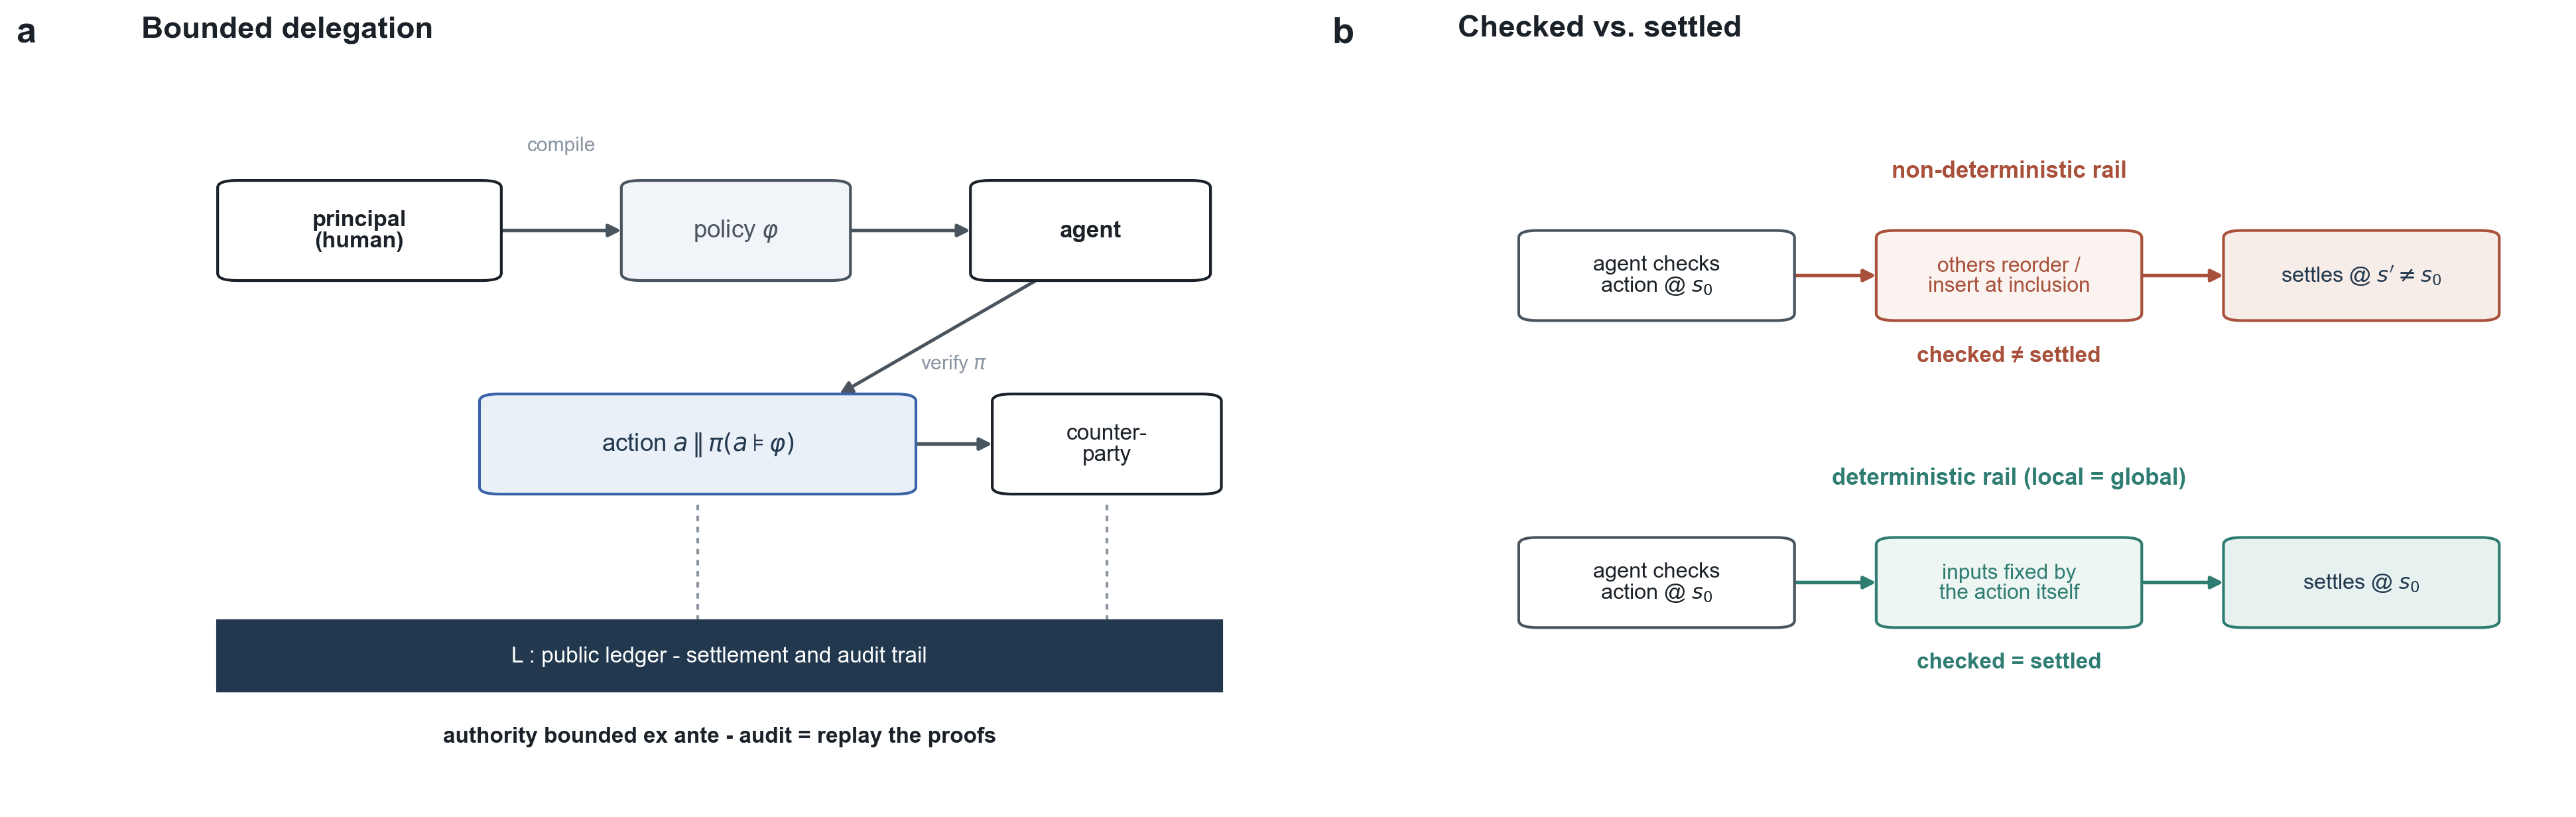
\includegraphics[width=\textwidth]{fig2_delegation.png}
  \caption{Bounded delegation and the determinism gap. \textbf{(a)}~A
    principal compiles policy $\varphi$; the agent's action $a$ travels
    with a proof $\pi(a \models \varphi)$ that the counterparty checks;
    settlement and audit reduce to replaying proofs against the public
    ledger $L$. Authority is bounded before the fact. \textbf{(b)}~Why
    determinism (\R{2}) is load-bearing: on a non-deterministic rail,
    reordering or insertion between check and inclusion settles a state
    $s' \neq s_0$, so the agent's verified action is not the one that
    settles; on a deterministic rail the action's inputs fix its effect,
    and checked equals settled. Schematic.}
  \label{fig:delegation}
\end{figure}

This is not a forecast about how agents \emph{might} transact; it is, in
outline, how the first standards already say they will. The agent-payment
protocols now shipping anchor each purchase to a chain of signed mandates
precisely so that authorisation rests on verifiable intent rather than on
a model's say-so \citep{ap2google2025,x402coinbase2025}, and account
abstraction supplies the bounded, revocable credential the mandate
authorises against \citep{erc4337}. What they do not yet supply is the
substrate guarantee of \R{2}: most settle on account-model rails where
the checked action and the settled action can still diverge
\citep{daian2020flashboys}. The demand side of the complement is being
built in the open; the determinism that would make it safe at machine
speed is the half still missing, and \S\ref{sec:open} treats it as the
live test it is.

Identity resolves along the same line. The question a counterparty must
answer---\emph{what is this, and who stands behind it?}---splits into
checkable predicates. Personhood, where it is required, becomes something
an actor can prove rather than assert \citep{borge2017personhood};
agent credentials chain back to an accountable principal through
signatures whose origin is itself checkable \citep{diffie1976new};
and the provenance of what an agent produces can travel with it as a
signed claim rather than a guess for a detector to second-guess
\citep{c2pa2024}. In each case the move is the same as the move that
defines the whole architecture: replace an after-the-fact judgement about
a fluent artifact with a before-the-fact proof attached to it.

Two observations follow. The first is about cost. Humans experience this
machinery as friction---keys, wallets, attestations, a worse experience
than simply being trusted---which is why human-facing crypto has
struggled to matter. Agents experience the opposite: reputation is a
thing they cannot natively hold, while generating and checking proofs is
what they do at native speed, and they do not tire, do not misread an
address, and cannot be socially engineered through a substrate that
admits only valid actions. The friction that repels human users is
weightless to the population now arriving. The second is about direction
of fit. Generative AI is the demand: it produces decisions faster than
any trusted human apparatus can vet them. Verifiable, deterministic
settlement is the only supply response whose throughput scales with
compute rather than with attention. The two are not rivals competing for
the same narrative slot; one makes decisions abundant, the other makes
them bind---and a decision that cannot bind is, economically, just
talk.

\section{Open Problems and Disconfirmation}
\label{sec:open}

The thesis is a technical bet, and an honest bet names both its unsolved
parts and the evidence that would settle it against us.

Four problems are open. \emph{Cost and latency}: proving every action is
not free, and an agent transacting continuously may generate proofs
faster than they can be produced or verified cheaply; whether
proof-bearing settlement can meet machine-speed commerce at acceptable
cost is unresolved, and recursive composition (\R{3}) is a partial answer,
not a finished one. \emph{Governance} (\R{5}): self-amendment inside the
verified record is young, thinly participated in, and already strained;
no system has shown that a constitution can evolve a proof language and
a fee policy without either capture or paralysis. \emph{The predicate
problem}: a mandate is only as good as the policy $\varphi$ a principal
can actually express, and writing $\varphi$ for open-ended conduct---
anticipating what an agent must never do---may be as hard as the
alignment problem it resembles; the substrate enforces $\varphi$, it does
not author it. \emph{Bootstrapping}: the constraint layer is most useful
once agents and counterparties already use it, the classic adoption
trap, and architectural fitness does not dissolve it.

Four observations would disconfirm the account. The earliest
agent-payment standards already settle on non-deterministic rails
\citep{x402coinbase2025}; if agent commerce stays there at scale and over
time, untroubled by the extractable-value tax \citep{daian2020flashboys},
then \R{2} is wrong about what agents will pay to avoid, and determinism
is not load-bearing.
If provenance and agent identity consolidate into a handful of platform
attestation services---device makers, app stores, model
providers---then the ownerless substrate (\R{4}) has lost to a
recentralised one, and the testimony regime is simply rebuilt at higher
concentration with root keys; this is, in our view, the likeliest way the
thesis fails, and it is a question of market structure, not of
feasibility. If advances make agents bindable \emph{internally}---
hardware-attested, verifiable execution carried within the model stack
itself---then the external substrate is redundant and the complement
dissolves. And if, among open substrates, the share of fees paid for
settlement, proving, and attestation never overtakes the share paid for
speculative turnover, then these systems are venues rather than
infrastructure, whatever their design---a test the case of
\S\ref{sec:case} is deliberately not exempt from.

\section{Coda: Who Writes the Rule}
\label{sec:coda}

The division of labour is the whole of the argument. A generative model
supplies decision; a deterministic, proof-bearing, ownerless substrate
supplies consequence; together they make an autonomous actor that can be
delegated to, bounded, and held to account---which neither half can be
alone. This is not a story about machines replacing institutions. It is a
story about rebuilding, for non-human actors, the thing institutions did
for human ones: convert a decision into a commitment that binds.

One faculty appears on neither side of the division. The substrate
enforces the policy $\varphi$; the agent acts within it; but the choice
of $\varphi$---what an agent must never do, what counts as compliant,
which outcomes are worth making irreversible---is authored by neither.
Writing the rule is not a task an agent can be delegated, because it is
the act that defines the bounds of every delegation beneath it; and it is
not a computation the substrate performs, because the substrate only
checks. It is the authorship of constraint, and it stays with whoever
bears the consequence of getting it wrong. As decision grows abundant and
its settlement grows automatic, the scarce and consequential act is no
longer deciding, and no longer enforcing. It is saying, in advance and on
the record, what shall and shall not be allowed to bind.

\paragraph*{Data availability.}
This is a theoretical contribution; it reports no experiment and no
empirical dataset. All claims rest on the cited literature; the scripts
and materials that regenerate the figures are released with the code.

\paragraph*{Code availability.}
Both figures are schematic and are generated by the released script at
\url{https://github.com/xinhao-zheng/constraint-layer}; no empirical
series is plotted.

\paragraph*{Author contributions.}
X.Z. conceived the argument, designed the figures, and wrote the
manuscript.

\paragraph*{Competing interests.}
The author holds no position in any asset discussed and received no
funding from any entity named.

\paragraph*{Ethics note.}
No human subjects were involved. System and product names are used
descriptively; the case analysis is architectural and is not investment
guidance.

\begin{thebibliography}{27}
\small\setlength{\itemsep}{2pt}
% Entries ordered by first citation in the text.

\bibitem[North(1990)]{north1990institutions}
North, D.~C. (1990). \emph{Institutions, Institutional Change and
Economic Performance}. Cambridge University Press.

\bibitem[Arrow(1974)]{arrow1974limits}
Arrow, K.~J. (1974). \emph{The Limits of Organization}. Norton, New York.

\bibitem[Park et~al.(2023)]{park2023generative}
Park, J.~S., O'Brien, J.~C., Cai, C.~J., Morris, M.~R., Liang, P., and
Bernstein, M.~S. (2023). Generative agents: Interactive simulacra of
human behavior. In \emph{UIST 2023}. ACM.

\bibitem[Chan et~al.(2023)]{chan2023harms}
Chan, A., Salganik, R., Markelius, A., et~al. (2023). Harms from
increasingly agentic algorithmic systems. In \emph{ACM FAccT 2023},
pages 651--666.

\bibitem[Sadasivan et~al.(2023)]{sadasivan2023detection}
Sadasivan, V.~S., Kumar, A., Balasubramanian, S., Wang, W., and Feizi, S.
(2023). Can {AI}-generated text be reliably detected? arXiv:2303.11156.

\bibitem[Zhang et~al.(2023)]{zhang2023watermarks}
Zhang, H., Edelman, B.~L., Francati, D., Venturi, D., Ateniese, G., and
Barak, B. (2023). Watermarks in the sand: Impossibility of strong
watermarking for generative models. arXiv:2311.04378.

\bibitem[Necula(1997)]{necula1997pcc}
Necula, G.~C. (1997). Proof-carrying code. In \emph{POPL~'97}, pages
106--119. ACM.

\bibitem[Goldwasser et~al.(1989)]{goldwasser1989knowledge}
Goldwasser, S., Micali, S., and Rackoff, C. (1989). The knowledge
complexity of interactive proof systems. \emph{SIAM Journal on
Computing}, 18(1):186--208.

\bibitem[Ben-Sasson et~al.(2014)]{bensasson2014zerocash}
Ben-Sasson, E., Chiesa, A., Garman, C., Green, M., Miers, I., Tromer, E.,
and Virza, M. (2014). Zerocash: Decentralized anonymous payments from
{Bitcoin}. In \emph{IEEE Symposium on Security and Privacy}, pages
459--474.

\bibitem[Google et~al.(2025)]{ap2google2025}
Google and partners (2025). \emph{Agent Payments Protocol (AP2): An Open
Protocol for Agent-Led Payments}. Technical specification, September 2025.

\bibitem[Coinbase and Cloudflare(2025)]{x402coinbase2025}
Coinbase and Cloudflare (2025). \emph{x402: An Open Standard for
Internet-Native Payments over {HTTP} 402}. x402 Foundation.

\bibitem[Buterin et~al.(2021)]{erc4337}
Buterin, V., Weiss, Y., Tirosh, D., Nacson, S., and Forshtat, A. (2021).
{ERC-4337}: Account abstraction using an alt mempool. Ethereum
Improvement Proposals.

\bibitem[Szabo(1997)]{szabo1997formalizing}
Szabo, N. (1997). Formalizing and securing relationships on public
networks. \emph{First Monday}, 2(9).

\bibitem[Catalini and Gans(2020)]{catalini2020simple}
Catalini, C. and Gans, J.~S. (2020). Some simple economics of the
blockchain. \emph{Communications of the ACM}, 63(7):80--90.

\bibitem[Kiayias et~al.(2017)]{kiayias2017ouroboros}
Kiayias, A., Russell, A., David, B., and Oliynykov, R. (2017). Ouroboros:
A provably secure proof-of-stake blockchain protocol. In \emph{CRYPTO
2017}, LNCS 10401, pages 357--388. Springer.

\bibitem[David et~al.(2018)]{david2018praos}
David, B., Ga\v{z}i, P., Kiayias, A., and Russell, A. (2018). Ouroboros
Praos: An adaptively-secure, semi-synchronous proof-of-stake blockchain.
In \emph{EUROCRYPT 2018}, LNCS 10821, pages 66--98. Springer.

\bibitem[Daian et~al.(2020)]{daian2020flashboys}
Daian, P., Goldfeder, S., Kell, T., Li, Y., Zhao, X., Bentov, I.,
Breidenbach, L., and Juels, A. (2020). Flash boys 2.0: Frontrunning in
decentralized exchanges, miner extractable value, and consensus
instability. In \emph{IEEE Symposium on Security and Privacy}, pages
910--927.

\bibitem[Chakravarty et~al.(2020)]{chakravarty2020eutxo}
Chakravarty, M. M.~T., Chapman, J., MacKenzie, K., Melkonian, O.,
Peyton~Jones, M., and Wadler, P. (2020). The extended {UTXO} model. In
\emph{Financial Cryptography Workshops (WTSC)}, LNCS 12063, pages
525--539. Springer.

\bibitem[Chakravarty et~al.(2021)]{chakravarty2021hydra}
Chakravarty, M. M.~T., Coretti, S., Fitzi, M., Ga\v{z}i, P., Kant, P.,
Kiayias, A., and Russell, A. (2021). Hydra: Fast isomorphic state
channels. Cryptology ePrint Archive, Report 2020/299.

\bibitem[Kerber et~al.(2021)]{kerber2021kachina}
Kerber, T., Kiayias, A., and Kohlweiss, M. (2021). Kachina: Foundations
of private smart contracts. In \emph{IEEE Computer Security Foundations
Symposium}, pages 47--62.

\bibitem[Midnight(2024)]{midnight2024}
Midnight Foundation (2024). \emph{Midnight: A Data-Protection
Blockchain---Technical Overview}. Project documentation.

\bibitem[Nakamoto(2008)]{nakamoto2008}
Nakamoto, S. (2008). Bitcoin: A peer-to-peer electronic cash system.
White paper.

\bibitem[Br\"unjes et~al.(2020)]{brunjes2020rewards}
Br\"unjes, L., Kiayias, A., Koutsoupias, E., and Stouka, A.-P. (2020).
Reward sharing schemes for stake pools. In \emph{IEEE European Symposium
on Security and Privacy}, pages 256--275.

\bibitem[CIP-1694(2023)]{cip1694}
Cardano community (2023). \emph{CIP-1694: An On-Chain Decentralized
Governance Mechanism for Voltaire}. Cardano Improvement Proposals.

\bibitem[Borge et~al.(2017)]{borge2017personhood}
Borge, M., Kokoris-Kogias, E., Jovanovic, P., Gasser, L., Gailly, N., and
Ford, B. (2017). Proof-of-personhood: Redemocratizing permissionless
cryptocurrencies. In \emph{IEEE EuroS\&P Workshops}, pages 23--26.

\bibitem[Diffie and Hellman(1976)]{diffie1976new}
Diffie, W. and Hellman, M.~E. (1976). New directions in cryptography.
\emph{IEEE Transactions on Information Theory}, 22(6):644--654.

\bibitem[C2PA(2024)]{c2pa2024}
Coalition for Content Provenance and Authenticity (2024). \emph{C2PA
Technical Specification, v2.0}. Standard.

\end{thebibliography}

\end{document}
